

\chapter{Symplectic Integration}
\label{cha:ham}

\section{Hamiltonian Systems and Numerical Methods}

\subsection{Hamiltonian Dynamics}

A Hamiltonian system on $(q,p)$ \cite{gni2006} is given by
\begin{align*}
	&\dot{q} = \dfrac{\partial H}{\partial p}
	&
	\dot{p} = \dfrac{-\partial H}{\partial q}&.	
\end{align*}
We use $q$ to denote position, and $p$ to denote momentum.
This is a special form of a general system of ODEs $\dot{x} = f(t,x)$.
For this part of our discussion, we will primarily be concerned with \textit{autonomous} systems of the form $\dot{x} = f(x)$.

We describe a system with its Hamiltonian $H(q,p)$, used to describe the total energy present.
We can write the system as
\begin{equation}
	\dfrac{\mathrm{d}}{\mathrm{d}t}\begin{pmatrix}
		q \\
		p
	\end{pmatrix} = \begin{bmatrix}
		\strut 0 & \strut 1 \\
		\strut -1 & \strut 0
	\end{bmatrix}\begin{bmatrix}
	\dfrac{\strut \partial H}{\strut\partial q} \\
	\dfrac{\strut \partial H}{\strut\partial p}
	\end{bmatrix}.
\end{equation}
If we write $x = (q,p)^\top$ and denote the matrix as $J$,
then the statement of a Hamiltonian system is of the form 
\begin{equation}
	{\dot{x}} = {J}\nabla H({x}).
	\label{eqn:hdyn}
\end{equation}
We call $J$ the \textit{symplectic matrix}.
The Hamiltonian is a first integral of the system

For a $d$-dimensional problem,
we instead denote the variables $q_1, \mathellipsis, q_n, p_1, \mathellipsis, p_n$ as the position and momentum in the directions of each basis vector respectively.
Write $x = (q_1, \mathellipsis, q_n, p_1, \mathellipsis, p_n)$.
Define $J$ to be the matrix defined in blocks
\begin{equation}
	J = \begin{bmatrix}
		{0}_n & {I}_n \\
		-{I}_n & {0}_n
	\end{bmatrix}
\end{equation}
and the problem can be written as ${\dot{x}} = {J}\nabla H({x})$.
This is the general form for a Hamiltonian system.
Note that for a problem in $d$ dimensions,
$x$ belongs to $\mathds{R}^{2d}$.
The $\nabla$ operator is specifically defined in the $(q,p)$ order for our purposes
\begin{equation*}
	\nabla = \begin{pmatrix}
		\frac{\partial}{\partial q_1} \\
		\vdots \\
		\frac{\partial}{\partial q_d} \\
		\frac{\partial}{\partial p_1} \\
		\vdots \\
		\frac{\partial}{\partial q_d}
	\end{pmatrix}
\end{equation*}

\subsection{The Simple Harmonic Oscillator}

First, we look at the simple harmonic oscillator $m \ddot{x} = -k x$.
In Hamiltonian variables this is
\begin{equation*}
	\begin{aligned}
		&\dot{q} = \frac{p}{m}, &\dot{p} = m\ddot{q} = -kq.
	\end{aligned}
\end{equation*}
A suitable Hamiltonian \cite{Casas_2016} is
\begin{equation*}
	H = \frac{1}{2m}p^2 + \frac{1}{2}kq^2.
\end{equation*}
Applying the forward Euler method to the problem, we get
\begin{equation*}
	\begin{aligned}
		q_{n+1} &= q_n + h\frac{\partial H}{\partial p}(q_n, p_n) &= q_n + \frac{p_n}{m}\\
		p_{n+1} &= p_n - h\frac{\partial H}{\partial q}(q_n, p_n) &= p_n - kq_n
	\end{aligned}
\end{equation*}
which can be written as a matrix equation
\begin{equation*}
	\begin{pmatrix}
		q_{n+1} \\
		p_{n+1}
	\end{pmatrix} = \begin{bmatrix}
		1 & 1/m \\
		-k & 1
	\end{bmatrix} \begin{pmatrix}
		q_n \\
		p_n
	\end{pmatrix}.
\end{equation*}
The matrix defines a map from one value of the numerical solution to the next.
We can consider a similar concept for the true solution of the problem, called the \textit{flow}.

\subsection{The Flow Map}

\begin{definition}
	The flow $\varphi_t$ is a map of the system from an initial time to the time $t$.
	Specifically, we write $\varphi_t(\alpha) = {x}(t)$ given the initial condition ${x}(t=0) = \alpha$.
	Hence the flow $\varphi_t:\mathds{R}^{2d}\rightarrow \mathds{R}^{2d}$ is a map from the initial point of the system to the time $t$.
\end{definition}
The Jacobian matrix $\varphi'_t({\alpha})$ is often called the sensitivity of the flow.
It describes the relative change in the problem per change in initial conditions.
We show the element-wise expression: %marcus said to change this
\begin{align*}
	\left[ \varphi'_t(\alpha) \right]_{ij} &= \left[ \frac{\partial }{\partial \alpha} \varphi_t(\alpha) \right]_{ij} \\
	&= \left[ \frac{\partial }{\partial \alpha} x(t) \right]_{ij} \\
	&= \frac{\partial x_i(t)}{\partial \alpha_j} \\
\end{align*}
for $i, j = 1, \mathellipsis, 2d$, which is the Jacobian matrix.
\begin{definition}
	A flow is symplectic if it satisfies $\varphi'_t(\alpha)^\top {J} \varphi'_t(\alpha) = {J}$,
	where $J$ is the symplectic matrix.
\end{definition}
Along with the flow of the system, we must consider the \textit{numerical flow},
which is the map from $x_n$ to $x_{n+1}$ defined by a numerical method.
\begin{definition}
	A numerical method defines a flow map $\Psi_h$ by
	\begin{equation*}
		x_{n+1} = \Psi_h(x_n).
	\end{equation*}
\end{definition}
The sensitivity of the numerical flow is affected similarly by a change in initial conditions. %ummmm
However, due to the discrete form of a numerical solution we will not give a general form.
The sensitivity of the numerical flow map can however be written explicitly when applying a given method to a given problem.

\subsection{Symplectic Flow}

The flow of a Hamiltonian system is, by definition, symplectic.
Recall the example of the simple harmonic oscillator.
We can demonstrate symplecticity with the actual flow map. Note the general closed form solution:
\begin{equation*}
	\begin{aligned}
		q(t) &= A\cos\left( \sqrt{\frac{k}{m}} t \right) + B \sin\left( \sqrt{\frac{k}{m}}t \right) \\
		p(t) &= B\sqrt{km} \cos\left( \sqrt{\frac{k}{m}} t \right) -A\sqrt{km} \sin\left( \sqrt{\frac{k}{m}}t \right) 
	\end{aligned}
\end{equation*}
for arbitrary constants $A$ and $B$.
Impose initial conditions:
suppose $q(t=0) = q_0,~ p(t=0) = p_0.$
Define $\omega = \sqrt{k/m}$ for shorthand, and apply the initial conditions to find that the coefficients are $A = q_0,~ B = p_0/m \omega$
Hence the particular solution is
\begin{equation*}
	\begin{aligned}
		q(t) &= q_0 \cos\left( \omega t \right) + \frac{p_0}{m\omega} \sin\left( \omega t \right) \\
		p(t) &= p_0 \cos\left( \omega t \right) - q_0 m\omega \sin\left( \omega t \right).
	\end{aligned}
\end{equation*}
We are in the position to evaluate the Jacobian entry-wise.
\begin{equation*}
	\varphi'_t \begin{pmatrix}
		q_0 \\
		p_0
	\end{pmatrix} = \begin{bmatrix}
		\frac{\partial q}{\partial q_0} & \frac{\partial q}{\partial p_0} \\
		\frac{\partial p}{\partial q_0} & \frac{\partial p}{\partial p_0}
	\end{bmatrix} = \begin{bmatrix}
		\cos(\omega t) & \frac{1}{m\omega} \sin(\omega t) \\
		-m\omega \sin(\omega t) & \cos(\omega t)
	\end{bmatrix},
\end{equation*}
and if we now plug this into the symplectic identity we get
\begin{align*}
	\varphi'_t(x_0)^\top {J} \varphi'_t(x_0) &= \begin{bmatrix}
		\cos(\omega t) & -m\omega \sin(\omega t) \\
		\frac{1}{m\omega} \sin(\omega t) & \cos(\omega t)
	\end{bmatrix} \begin{bmatrix}
		0 & 1 \\
		-1 & 0
	\end{bmatrix} \begin{bmatrix}
		\cos(\omega t) & \frac{1}{m\omega} \sin(\omega t) \\
		-m\omega \sin(\omega t) & \cos(\omega t)
	\end{bmatrix} \\
	&= \begin{bmatrix}
		m \omega \sin(\omega t) & \cos(\omega t) \\
		-\cos(\omega t) & \frac{1}{m \omega} \sin(\omega t)
	\end{bmatrix} \begin{bmatrix}
		\cos(\omega t) & \frac{1}{m\omega} \sin(\omega t) \\
		-m\omega \sin(\omega t) & \cos(\omega t)
	\end{bmatrix} \\
	&= \begin{bmatrix}
		m \omega \sin(\omega t) \cos(\omega t) - m \omega \sin(\omega t) \cos(\omega t)  & \sin^2(\omega t) + \cos^2(\omega t) \\
		-\cos^2(\omega t) - \sin^2(\omega t) & -\frac{1}{m\omega}\cos(\omega t)\sin(\omega t) + \frac{1}{m \omega}\cos(\omega t)\sin(\omega t)
	\end{bmatrix} \\
	&= \begin{bmatrix}
		0 & 1 \\
		-1 & 0
	\end{bmatrix} = {J}.
\end{align*}
Hence the flow is symplectic.

\subsection{A symplectic integrator}

With symplectic integration, we are interested in numerical methods for which the numerical flow also attains symplecticity.
One such example is the symplectic Euler method \cite{gni2006} given by
\begin{equation*}
	\begin{pmatrix}
		q_{n+1} \\
		p_{n+1} 
	\end{pmatrix} = \begin{pmatrix}
		q_{n} \\
		p_{n}
	\end{pmatrix} + h \nabla H(q_{n}, p_{n+1}).
\end{equation*}
For an arbitrary problem this method is implicit. However, many problems have a separate Hamiltonian that allows the iteration to be performed in two explicit steps. 
The simple harmonic oscillator has a Hamiltonian $H(q, p) = \frac{1}{2m}p^2 + \frac{1}{2}kq^2$ which can be written as $H(q, p) = V(q) + T(p)$, where $V(q)$ represents kinetic energy and $T(p)$ represents potential energy of the system \cite{gni2006, Casas_2016}.
We expand out the method as
\begin{equation*}
	\begin{pmatrix}
		q_{n+1} \\
		p_{n+1} 
	\end{pmatrix} = \begin{pmatrix}
		q_{n} \\
		p_{n}
	\end{pmatrix} + h {J} \begin{pmatrix}
		V'(q_n) \\
		T'(p_{n+1})
	\end{pmatrix} = \begin{pmatrix}
		q_{n} + \frac{h}{m}p_{n+1} \\
		p_{n} - hk q_n
	\end{pmatrix}.
\end{equation*}
On inspection, we can perform this iteration separably: compute $p_{n+1}$ using $p_n$ and $q_n$,
then use $q_n$ and $p_{n+1}$ to compute $q_{n+1}$.
Important to note is that this is specifically the symplectic Euler-VT method, since we evaluate $V'$ and then $T'$,
and the symplectic Euler-TV method is an alternative which computes in the opposite order analogously.
This is of course assuming that the Hamiltonian is separable, which it may not be.
For simplicity we will stick with the VT method for examples.
We find an expression for the numerical flow:
\begin{equation*}
	\begin{aligned}
		\begin{pmatrix}
			q_{n+1} \\
			p_{n+1} 
		\end{pmatrix} &= \begin{pmatrix}
			q_{n} + \frac{h}{m} \left( p_{n} - h \omega q_n \right) \\
			p_{n} - h \omega q_n
		\end{pmatrix} \\
		&= \begin{bmatrix}
			1 - \frac{h^2 k}{m} & \frac{h}{m} \\
			-hk & 1
		\end{bmatrix} \begin{pmatrix}
			q_n \\
			p_n
		\end{pmatrix} \equiv \Phi_h \begin{pmatrix}
			q_n \\
			p_n
		\end{pmatrix}
	\end{aligned}
\end{equation*}
and just like before, test the symplectic identity
\begin{equation*}
	\Phi^\top{J}\Phi = \begin{bmatrix}
		\left(1-\frac{h^2 k}{m}\right)(-hk) + \left(\frac{h^2 k}{m}-1\right)(-hk) & 1 - \frac{h^2 k}{m} + \frac{h^2 k}{m} \\
		-\frac{h^2 k}{m} + \frac{h^2 k}{m} -1 & \frac{h}{m} - \frac{h}{m}
	\end{bmatrix} = \begin{bmatrix}
		0 & 1 \\
		-1 & 0
	\end{bmatrix} = {J}.
\end{equation*}
Hence this method is symplectic for this example.

\section{Further Hamiltonian Dynamics}

\subsection{Derivatives of Flow Maps}

The flow map $\varphi_t: {x}_0 \rightarrow {x}(t)$ gives us powerful insights into the behaviour of Hamiltonian integration.
Before giving a result on the symplecticity of Hamiltonian systems, we need some results on flow maps.
We will show expressions for the time derivatives of $\varphi_t(\alpha)$ and $\varphi'_t(\alpha)$.
Starting with the flow, its time derivative is
\begin{align*}
	\frac{\mathrm{d}}{\mathrm{d}t} \left( \varphi_t({x}_0) \right) &= \frac{\mathrm{d}}{\mathrm{d}t} {x}(t) \\
	&= \dot{{x}}(t) \\
	&= {J}\nabla H({x}(t)) \\
	&= {J}\nabla H \left( \varphi_t({x}_0) \right).
\end{align*}
We have a similar form for the time derivative of the sensitivity:
\begin{align*}
	\frac{\mathrm{d}}{\mathrm{d}t} \left( \varphi'_t({x}_0) \right) &= \frac{\partial}{\partial {x}_0} \frac{\mathrm{d}}{\mathrm{d}t} \varphi_t({x}_0) \\
	&= \frac{\partial}{\partial {x}_0} \frac{\mathrm{d}}{\mathrm{d}t} {x}(t) \\
	&= \frac{\partial}{\partial {x}_0} \dot{{x}}(t) \\
	&= \frac{\partial}{\partial {x}_0} {J}\nabla H({x}(t)) \\
	&= J \nabla^2 H({x}(t)) \left(\frac{\partial}{\partial {x}_0} {x}(t)\right) \\
	&= J \nabla^2 H(\varphi_t({x}_0))\varphi'_t({x}_0).
\end{align*}

\subsection{Symplectic Flow of a Hamiltonian System}

Earlier, we looked at the symplecticity of the flow of a particular Hamiltonian system.
We will now generalise this result to any Hamiltonian system.
Symplecticity of the flow is equivalent to the system itself being Hamiltonian.

\begin{theorem}
\label{thm:hamil}
A dynamical system is Hamiltonian if and only if its flow is symplectic.
\end{theorem}
\begin{proof}
$(\Rightarrow)$ Consider the flow of a Hamiltonian system at time $t=0$. By definition, $\varphi_t(x_0) = x(t)$ given $x(0) = x_0$,
therefore $\varphi_0(x_0) = x_0$. Hence the sensitivity at $t=0$ is $\varphi'_0(x_0) = I$ the identity matrix.
The symplectic identity is satisfied trivially: $(\varphi'_0(x_0))^\top J \varphi'_0(x_0) = IJI = J$.

Now, instead of finding an expression of the symplectic identity at time $t$,
we show that this quantity is unchanging in time.
By differentiating, the expression distributes by the product rule:
\begin{equation*}
	\frac{\mathrm{d}}{\mathrm{d}t} \left(
		\varphi'_t(x_0)^\top J \varphi'_t(x_0)
	\right) = \left(
		\frac{\mathrm{d}}{\mathrm{d}t} \varphi'_t(x_0)^\top
	\right) J \varphi'_t(x_0) + \varphi'_t(x_0)^\top J \left(
		\frac{\mathrm{d}}{\mathrm{d}t} \varphi'_t(x_0)
	\right).
\end{equation*}
We can find an expression for the derivative term:
\begin{align*}
	\frac{\mathrm{d}}{\mathrm{d}t} \varphi'_t(x_0) &= \frac{\mathrm{d}}{\mathrm{d}t} J \nabla H(\varphi_t(x_0)) \\
	&= J \nabla^2 H(\varphi_t(x_0)) \varphi'_t(x_0).
\end{align*}
Now plug this back in, becoming
\begin{align*}
	\frac{\mathrm{d}}{\mathrm{d}t} \left(
		\varphi'_t(x_0)^\top J \varphi'_t(x_0)
	\right) &= \left( J \nabla^2 H(\varphi_t)\varphi'_t \right)^\top J \varphi'_t 
	+ \varphi'_t J \left( 
		J \nabla^2 H(\varphi_t) \varphi'_t
  	\right) \\
	&= (\varphi'_t)^\top \nabla^2 H(\varphi_t)^\top J^\top J \varphi'_t
	+ (\varphi'_t)^\top J^2 \nabla^2 H(\varphi_t) \varphi'_t(x_0) \\
	&= (\varphi'_t)^\top \nabla^2 H(\varphi_t)^\top \varphi'_t - (\varphi'_t)^\top \nabla^2 H(\varphi_t) \varphi'_t
\end{align*}
since $J^\top J = I$ and $J^2 = -I$.
Under the assumption that the Hessian matrix $\nabla^2 H(\varphi_t)$ is symmetric,
this expression evaluates to zero and hence the symplectic identity is satisfied for all $t$ and we are done.

$(\Leftarrow)$ Assuming that the sensitivity satisfies the symplectic identity, we want to show that the system is Hamiltonian.
For a general system, we have $\dot{x} = f(x)$. We want to show that we can write $f(x) = J \nabla H(x)$ for some function $x$, in order for the system to be Hamiltonian.
The flow is symplectic, so it satisfies
\begin{equation*}
	\varphi'_t(x_0)^\top J \varphi'_t(x_0) = J. 
\end{equation*}
Differentiating this expression gives, similar to earlier,
\begin{equation*}
	\varphi'_t(x_0)^\top \frac{\partial f}{\partial x_0}(\varphi_t(x_0))^\top J \varphi'_t(x_0) + \varphi'_t(x_0)^\top J \frac{\partial f}{\partial x_0}(\varphi_t(x_0)) \varphi'_t(x_0) = 0.
\end{equation*}
By taking factors on the left and right, this is
\begin{equation*}
	\varphi'_t(x_0)^\top \left[ \frac{\partial f}{\partial x_0}(\varphi_t(x_0))^\top J + J \frac{\partial f}{\partial x_0}(\varphi_t(x_0)) \right] \varphi'_t(x_0) = 0.
\end{equation*}
This must be true for all $t$, so if we set $t=0$ the sensitivity matrix appearing on both the right and left is the identity.
Because $J = -J^\top$, we have that
\begin{equation*}
	\left[ J \frac{\partial f}{\partial x_0} \right]= \left[ J \frac{\partial f}{\partial x_0} \right]^\top
\end{equation*}
i.e. the matrix is symmetric. 
The required result is given in \cite{gni2006}, namely that $f(x)$ can be written in the form $J \nabla H(x)$.
\end{proof}

We now properly understand the link between Hamiltonian mechanics and symplectic integration.
The formal definition for a symplectic integrator is that the method maintains the form $\mathrm{d}q_i \wedge \mathrm{d}p_i$ with $i = 1, \mathellipsis, d$ for an $d$-dimensional problem \cite{gni2006}.
The form is an infinitesimal area generated by the infinitesimals in $q, p$.
For a one-dimensional problem, we can produce the phase portrait by plotting $p$ against $q$.
A single point in the phase portrait represents the state of the dynamical system at a fixed point in time.
The flow and the numerical flow are maps between points in the phase portrait.
If we think of the phase portrait as a solution space for a one-dimensional dynamical system, we can say that symplectic methods preserve the area of the solution space.
This is the paradigm of symplectic integration: by maintaining area of the phase space under mapping of the numerical flow, we maintain qualitative behaviour of the ODE over long timespans.
Furthermore, the conservation of area is equivalent to a symplectic method maintaining a first integral of the system, which is the Hamiltonian $H$.
We will however make it clear that a symplectic integrator does not exactly preserve the Hamiltonian of the problem, this being something we will explore in more detail.

In order to apply a symplectic integration method to a problem, we need an expression for the Hamiltonian of that problem,
and we need a numerical method for which the symplecticity of the flow is preserved.

\subsection{The Simple Pendulum}

%figure on comparison of three methods

\begin{figure}
	\centering
	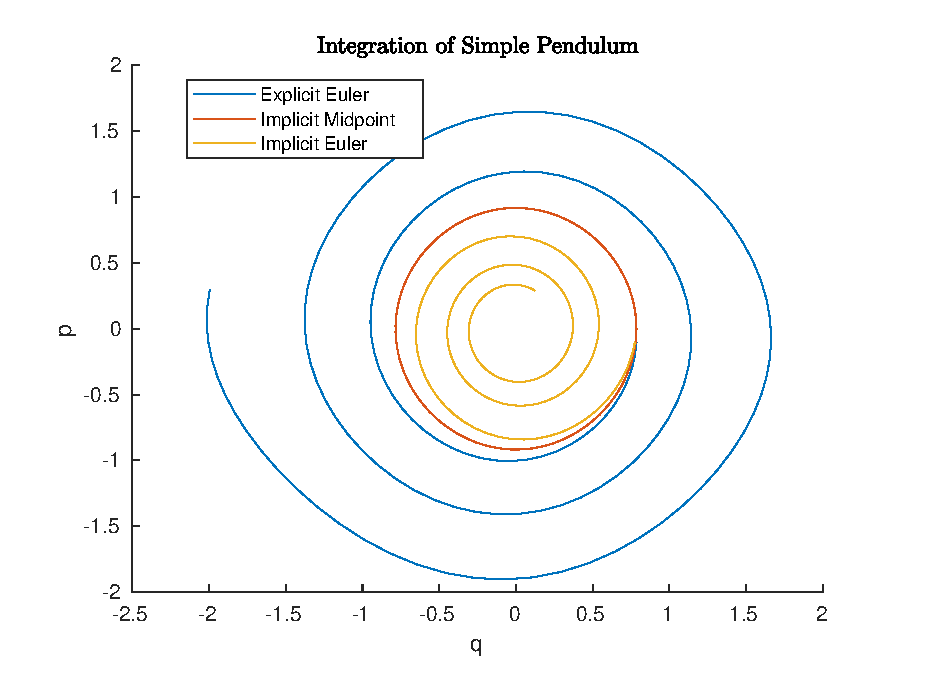
\includegraphics[width=0.66\linewidth]{figures/pendulum.eps}
	\caption{
		Integration of the simple pendulum as a Hamiltonian mechanics problem, plotted as a phase portrait.
		The explicit Euler method gradually diverges, a consequence of it lacking A-stability.
		The implicit Euler method converges to zero.
		Using implicit midpoint, we stay on the path followed by the pendulum, since this method is symplectic.
	}
	\label{fig:pendulum}
\end{figure}

The simple pendulum is the one-dimensional system defined by
\begin{equation*}
	ml\frac{\mathrm{d}^2 \theta}{\mathrm{d}t^2} = - mg \sin(\theta)
\end{equation*}
For this problem, we define $q = \theta$, $p = \dot{\theta}$ and the Hamiltonian \cite{Casas_2016} as
\begin{equation*}
	H(q,p) = \frac{1}{2}p^2 + k^2(1-\cos(q))
\end{equation*}
where $k^2 = g/l$.
This Hamiltonian can be obtained by integrating the system, and is therefore a conserved quantity.
We will look at a selection of numerical methods applied to this problem.
Recall Euler's method, which takes the form $x_{n+1} = x_n + h {J} \nabla H(x_n)$ for a Hamiltonian system.
This expands to:
\begin{equation*}
	\begin{pmatrix}
		q_{n+1} \\
		p_{n+1}
	\end{pmatrix}^E = \begin{pmatrix}
		q_n \\
		p_n
	\end{pmatrix} + h \begin{bmatrix}
		0 & 1 \\
		-1 & 0
	\end{bmatrix} \begin{pmatrix}
		k^2 \sin(q_n) \\
		p_n
	\end{pmatrix} = \begin{pmatrix}
		q_n + h p_n \\
		p_n - h k^2 \sin(q_n)
	\end{pmatrix}.
\end{equation*}
The Implicit Midpoint method gives us
\begin{equation*}
	\begin{pmatrix}
		q_{n+1} \\
		p_{n+1}
	\end{pmatrix}^M = \begin{pmatrix}
		q_n \\
		p_n
	\end{pmatrix} + h \begin{bmatrix}
		0 & 1 \\
		-1 & 0
	\end{bmatrix} \begin{pmatrix}
		k^2 \sin \left(\dfrac{q_n + q_{n+1}}{2}\right) \\
		\dfrac{p_n + p_{n+1}}{2}
	\end{pmatrix} = \begin{pmatrix}
		q_n + h \left( \dfrac{p_n + p_{n+1}}{2} \right) \\
		p_n - h k^2 \sin \left( \frac{q_n + q_{n+1}}{2} \right)
	\end{pmatrix}.
\end{equation*}
Finally, applying the Symplectic Euler-VT method yields
\begin{equation}
	\begin{pmatrix}
		q_{n+1} \\
		p_{n+1}
	\end{pmatrix}^S = \begin{pmatrix}
		q_n \\
		p_n
	\end{pmatrix} + h \begin{bmatrix}
		0 & 1 \\
		-1 & 0
	\end{bmatrix} \begin{pmatrix}
		k^2 \sin(q_n) \\
		p_{n+1}
	\end{pmatrix} = \begin{pmatrix}
		q_n + h p_{n+1} \\
		p_n - h k^2 \sin(q_n)
	\end{pmatrix}
\end{equation}
% change this since the figure uses implicit and explicit Euler and not symplectic euler.

See Figure \ref{fig:pendulum}, where we have applied three methods to the simple pendulum problem.
Only when applying the implicit midpoint method do the oscillations remain on a loop in the phase portrait.
The Symplectic Euler method is not shown, since it is identical to the result obtained from the implicit midpoint method.
The implicit midpoint method is a symplectic method, and probably the simplest to demonstrate.

Symplectic methods preserve the oscillation of the pendulum.
This means the pendulum oscillates consistently, without any drift.
In the explicit and implicit Euler methods, we observe a divergence or convergence of the bounds of oscillation respectively.
% not rigorous, ideally we prove that these methods are symplectic

It is important to note at the moment that the only examples we have looked at have closed form solutions.
Our results so far only serve for understanding the definition of symplecticity.
We now look at some stronger results about numerical methods.

\subsection{The Adjoint Flow Map}

We may now want to look at forming higher order symplectic methods. In order to do so, we need to consider generalised properties of flow maps which define these methods.
One such property is the \textit{adjoint} map.

\begin{definition}
	Given a method defined by a numerical flow $\Psi_h$,
	the adjoint $\Psi^*_h$ is the method that satisfies
	\begin{equation*}
		\Psi^*_{-h} = \Psi^{-1}_h.
	\end{equation*}
\end{definition}

In words, stepping backward with the adjoint method is equivalent to stepping forward with the inverse.
Adjoint methods are very useful. Given an arbitrary method $\Psi_h$,
the method $\Psi_{h/2} \circ \Psi_{h/2}^*$ is symmetric.
A symmetric method is a method that satisfies $\Psi_h^{-1} = \Psi_{-h}$.
This means if we integrate forwards in time by a particular step, and then integrate back,
we return to the original value since we are equivalently applying the inverse.
Time symmetric methods are geometric integrators themselves, preserving time symmetry,
however this is not something we will explore. % show that this composition is necessarily of even order

We can show that the implicit Euler method is the adjoint of explicit Euler \cite{sanz2018hamiltonian}.
First, let $\Psi_h^I$ denote the implicit method and let $\Psi_h^E$ denote the explicit method.
We want to show that $\Psi_h^E = (\Psi_{-h}^I)^{-1}$.
This is equivalent to $\Psi_{-h}^I \circ \Psi_h^E (x) = x$.
If we expand this composition, we obtain
\begin{align*}
	\Phi_{-h}^I \left( \Phi_j^E  (x) \right) &= \Phi_{-h}^I \left( x + h f(x) \right) \\
	&= x + h f(x) - h f\left( \Phi_{-h}^I \left( x + h f(x) \right) \right) \\
	&= x + h f(x) - h f\left( \Phi_{-h}^I \left( \Phi_h^E (x) \right) \right),
\end{align*}
and $\Phi_{-h}^I (\Phi_h^E (x)) = x$ solves this equation. Hence $(\Phi_{-h}^I)^{-1} = \Phi_h^E$.
Note that the explicit and implicit Euler methods cannot be symmetric because they are adjoint.

There are several properties of symplectic methods which may be of interest now.
We have not shown that ($1$) the adjoint of a symplectic method is symplectic, and ($2$) the composition of symplectic methods is symplectic.
These are relatively simple properties which can be proven from the defintions, but it will help our understanding to cover these.
\begin{proposition}
	The adjoint of a symplectic method is symplectic.
\end{proposition}
\begin{proof}
	First of all, the definition of the adjoint method states $\Phi^*_h = \Phi^{-1}_{-h}$.
	By algebraic manipulation,
	\begin{align*}
		\Phi_h^\top J \Phi_h &= J \\
		\Rightarrow \Phi_{-h}^\top J \Phi_{-h} &= J \\
		\Rightarrow J &= (\Phi_{-h}^{-1})^\top J (\Phi_{-h}^{-1}) = (\Phi_h^*)^\top J (\Phi_h^*)
	\end{align*}
	and so clearly the adjoint is symplectic.
\end{proof}
This result will be used in tandem with the composition of maps.
\begin{proposition}
	If $\Phi_h$ and $\Psi_h$ are two symplectic maps, then their composition $\Phi_h \circ \Psi_h$ is symplectic.
\end{proposition}
\begin{proof}
	This is done similarly. We have
	\begin{align*}
		\left(\Phi_h \Psi_h\right)^\top J \left(\Phi_h \Psi_h\right) &= \Psi_h^\top \Phi_h^\top J \Phi_h \Psi_h \\
		&= \Psi_h^\top J \Psi_h \\
		&= J.
	\end{align*}
	Therefore the composition of symplectic maps is symplectic.	
\end{proof}

We can now introduce a new method using these results.

\subsection{The St\"ormer-Verlet Method}

Earlier, we looked at the Symplectic Euler method, which is a modification of the Euler methods for Hamiltonian integration.
If the Hamiltonian is separable such that $H(q,p) = V(q) + T(p)$, then the Symplectic Euler method is explicit.
This is because in the Symplectic Euler-VT step, we use $p_n$ and $q_n$ to compute $p_{n+1}$, then use $p_{n+1}$ and $q_n$ to compute $q_{n+1}$.
This is exactly the method we applied in our earlier example introducing the Symplectic Euler method.
However, the Symplectic Euler method is generally implicit because a given Hamiltonian for a problem may not be separable.
Denote the Symplectic Euler step by $\Psi_h$. The \textit{St\"ormer-Verlet} method \cite{gni2006, Casas_2016} is defined by the step $\Psi_{h/2}^* \circ \Psi_{h/2}$.
Formally, this is
\begin{align*}
	p_{n+\frac{1}{2}} &= p_n - \frac{h}{2}\nabla_q H \left( q_n, p_{n+\frac{1}{2}} \right) \\
	q_{n+1} &= q_n + \frac{h}{2}\left( \nabla_p H \left( q_n, p_{n+\frac{1}{2}} \right) + \nabla_p H \left(q_{n+1}, p_{n+\frac{1}{2}} \right) \right) \\
	p_{n+1} &= p_{n+\frac{1}{2}} - \frac{h}{2} \nabla_q H \left( q_{n+1}, p_{n+\frac{1}{2}} \right).
\end{align*}
The St\"ormer-Verlet method is time-symmetric and second order accurate \cite{Casas_2016}.
We start with a step of the symplectic Euler method of length $h/2$, followed by its adjoint in which we step in $(q,p)$ in the opposite order.
This explains the structure where we have a step in $q$ of length $h$ in the middle of two steps in $p$ of length $h/2$.

We have defined the St\"ormer-Verlet method by the map $\Psi_{h/2}^* \circ \Psi_{h/2}$,
but we may also define a method as $\Psi_{h/2} \circ \Psi_{h/2}^*$,
which is an alternative St\"ormer-Verlet scheme which is also time-symmetric and second order.

The composition of a method with its adjoint leads to a method which is necessarily of even order \cite{sanz2018hamiltonian, hairerwanner1993, Casas_2016}.

\subsection{Mechanics}

% maybe send this bit to appendix
% talk about lagrangian and hamiltonian - canonical conjugate momentum
Before the next example, it helps to define context around the mechanics of Hamiltonian system,
In many cases, a Hamiltonian system has a Hamiltonian $H$ that we can express as $H(q,p) = T(p) + V(q)$.
The Hamiltonian is a conserved quantity of the system, such as the total energy being exchanged.
A \textit{Lagrangian} for a system can be defined as $L(q,p) = T(p) - V(q)$,
a difference in the energies.
The natural conjugate momentum is defined by
\begin{equation}
	p_k := \dfrac{\partial L}{\partial \dot{q}_k}
\end{equation}
for $k = 1,\mathellipsis,n$.
If we have a problem formulated generally, position is usually already defined.
Natural conjugate momentum means we can obtain an expression for momentum which aligns with the properties of Hamiltonian dynamics.
It often helps when defining and solving our own problems for the variables to be defined in this way.

\subsection{A Model for Phonation}

% figure on ODE45 vs a symplectic integrator for this problem, do the mobius-style figure

\begin{figure}
	\centering
	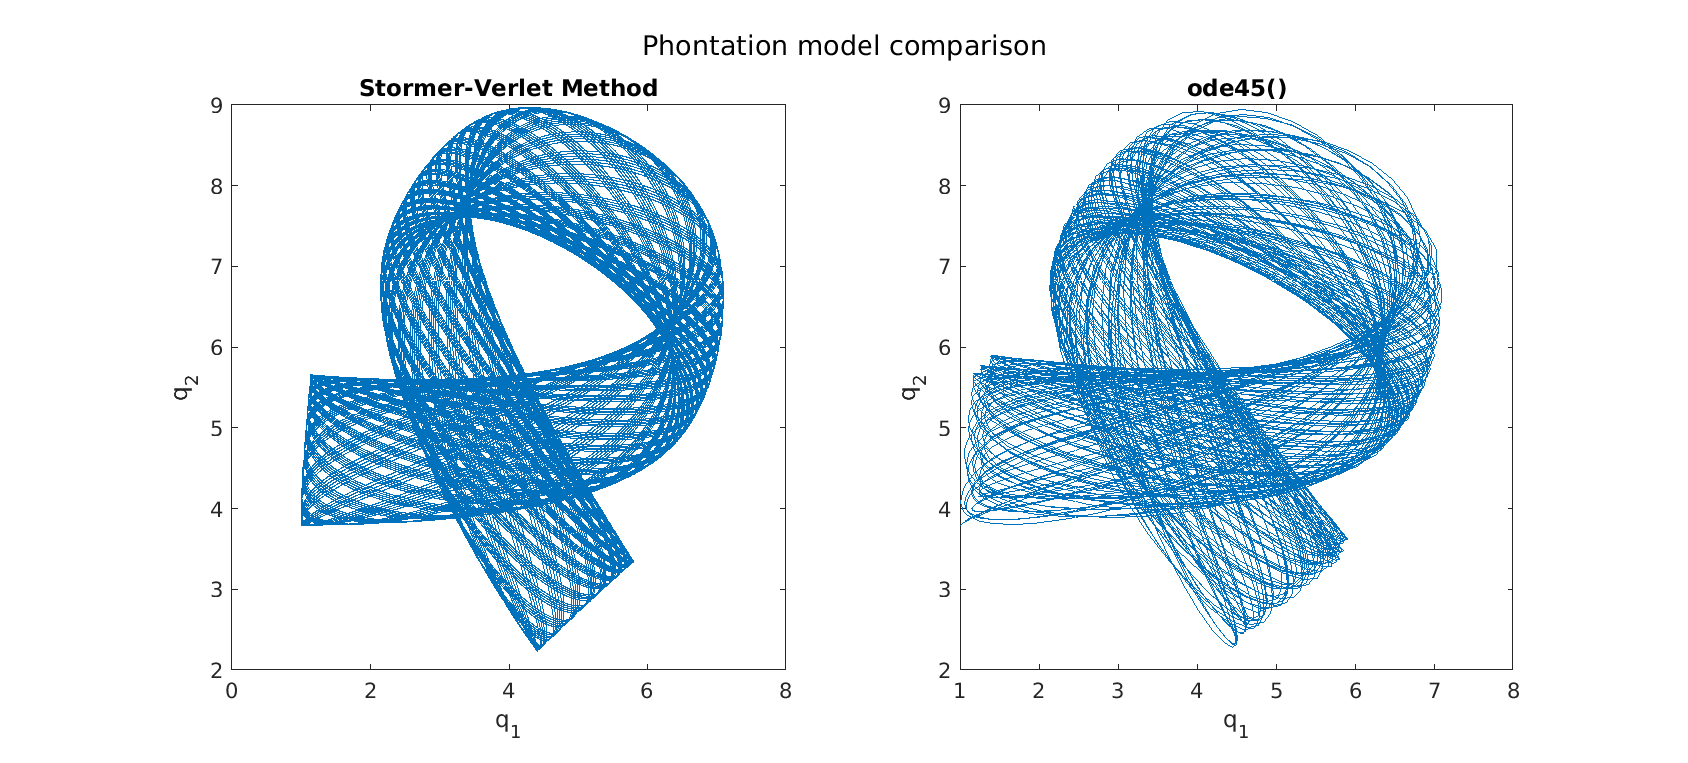
\includegraphics[width = \linewidth]{figures/phonationcomp.eps}
	\caption{
		Integration of the two mass model for phonation for $t \in [0, 1000]$.
		Figures show the oscillation bounds, plotting $q_2$ against $q_1$.
		In the left figure, we observe that a symplectic method retains the bounds of oscillation,
		whereas using \texttt{ode45()} the explicit Runge-Kutta method is not as well behaved and the bounds are not as clear. 
	}
	\label{fig:phon}
\end{figure}

This example is based on the two mass model from ``Models for Phonation''\footnote{
	\url{https://willwoolf.github.io/phon.pdf}
}.
A vocal cord is modelled by two stiffness-coupled masses, and their one-dimensional displacements are given by $u$ and $v$.
The governing equation for motion, from Newton's law, is
\begin{align*}
	\dfrac{\mathrm{d}^2 u}{\mathrm{d}t^2} &= 1 - u + \beta \left(1 - \dfrac{1}{u^2}\right) + \omega (v - u) \\
	\alpha \dfrac{\mathrm{d}^2 v}{\mathrm{d}t^2} &= \lambda(1 - v) + \beta \left(1 - \dfrac{1}{v^2}\right) + \omega (u - v)
\end{align*}
We first express this as a Hamiltonian problem. Denote $q_1 = u$, $q_2 = v$.
We define momentum $p_1 = \dot{q}_1$, $p_2 = \alpha \dot{q}_2$.
A Hamiltonian, obtained by integrating the system, is
\begin{equation*}
	H = \frac{1}{2} \left( p_1^2 + \frac{1}{\alpha} p_2^2 \right) + \frac{\omega}{2}(q_1 - q_2)^2 - F(q_1) - G(q_2)
\end{equation*}
where
\begin{align*}
	F(q_1) &= q_1 - \frac{1}{2}q_1^2 + \beta \left( q_1 + \frac{1}{q_1} \right) \\
	G(q_2) &= \lambda \left(q_2 - \frac{1}{2}q_2^2 \right) + \beta \left( q_2 + \frac{1}{q_2} \right).
\end{align*}
Therefore, in Hamiltonian variables the coupled ODEs can be expressed as
\begin{eqnarray*}
	\dot{q}_1 = p_1 & ~ & \dot{q}_2 = \frac{1}{\alpha} p_2 \\
	\dot{p}_1 = F'(q_1) - \omega(q_1 - q_2) & ~ & \dot{p_2} = G'(q_2) - \omega(q_2 - q_1)
\end{eqnarray*}
stating the problem in Hamiltonian form.
Since the Hamiltonian is a conserved quantity, we can use it to evaluate the behaviour of the integration method.
We can apply the Hamiltonian function to our numerical solutions, to verify that the quantity is in fact conserved by the numerical method.
A symplectic method does not preserve the Hamiltonian, but it preserves a particular Hamiltonian.
The closeness of this Hamiltonian can be shown via backward error analysis.
A regular integration method, such as an explicit Runge-Kutta scheme, will fail to preserve the Hamiltonian and the constant will diverge.
If the value changes by a significant amount, we can observe loss of qualitative behaviour.
Observe how, in Figure \ref{fig:phon}, we have shown an immediate comparison of the clarity of results from using a symplectic integrator,
versus using the efficient but not as stable explicit Runge-Kutta methods applied by MATLAB's \texttt{ode45()} integrator.

\section{Generalised Symplectic Methods}

\subsection{Conjugacy}

Before looking at more symplectic methods, we will cover a brief result on conjugacy of methods.
Consider the implicit midpoint and trapezium methods. Implicit midpoint is the method
\begin{equation*}
	\Phi_h^M (x_n) = x_{n+1} = x_n + hf\left(\frac{x_n + x_{n+1}}{2}\right).
\end{equation*}
The trapezium method is similar:
\begin{equation*}
	\Phi_j^T (x_n) = x_{n+1} = x_n + h \left(\frac{f(x_n) + f(x_{n+1})}{2}\right)
\end{equation*}
The implicit midpoint method is symplectic, but the trapezium method is not.
Interestingly, the trapezium method has excellent behaviour in preserving phase-space volume, despite not being a symplectic method.
It can be shown that these are conjugate methods \cite{sanz2018hamiltonian}, meaning that they exhibit similar long-term behaviour.
Two methods $\Psi_h, \Phi_h$ are conjugate if there exists a map $\chi$ such that $\Phi_h = \chi^{-1} \Psi_h \chi$.
Consider applying a method $\Phi_h$ $N$ times. Conjugacy shows that
\begin{align*}
	\left(\Phi_h\right)^N &= \left(\chi^{-1} \Psi_h \chi\right)^N \\
	&= \underbrace{\left(\chi^{-1} \Psi_h \chi \right)\left(\chi^{-1} \Psi_h \chi \right) \mathellipsis \left(\chi^{-1} \Psi_h \chi\right)}_{N} \\
	&= \chi^{-1} (\Psi_h)^N \chi.
\end{align*}
Therefore, conjugate methods remain separated by the conjugacy map $\chi$ for an arbitrary number of iterations.
%% find a defined inverse so that we can show conjugacy.

\subsection{Runge-Kutta Methods}

These are methods of the form
\begin{equation*}
	x_{n+1} = x_n + h \left( \sum_{i = 1}^{s} b_i k_i \right)
\end{equation*}
as defined in the introduction, equivalently defined by the Butcher tableau
\begin{equation*}
	\begin{array}{c|ccc}
		c &A \\
		\hline
		&b^\top .
	\end{array}
\end{equation*}
We will first consider A-stability.

Consider the linear test problem $\dot{x} = \lambda x$.
We have already explored stability for the basic Euler methods.
We will look at a general explicit 3-stage method.
\begin{example}
	First, find expressions for the $k_i$:
	\begin{align*}
		k_1 &= \lambda x_n, \\
		k_2 &= \lambda\left( x_n + h a_{21}k_1 \right) \\
		&= \left( \lambda + h a_{21}\lambda^2 \right)x_n, \\
		k_3 &= \lambda \left( x_n + h a_{31}k_1 + h a_{32}k_2 \right) \\
		&= \lambda \left( x_n + h a_{31} \lambda x_n + h a_{32}\left( \lambda + h a_{21} \lambda^2 \right) x_n \right) \\
		&= \left( \lambda + h a_{31}\lambda^2 + h a_{32}\lambda^2 + h^2 a_{32}a_{21}\lambda^3 \right) x_n.
	\end{align*}
	therefore
	\begin{align*}
		x_{n+1} &= x_n + h \left( b_1 k_1 + b_2 k_2 + b_3 k_3 \right) \\
		&= x_n + h b_1 \lambda x_n + h b_2 \left(\lambda + h a_{21} \lambda^2\right)x_n + hb_3 \left( \lambda + h a_{31} \lambda^2 + h a_{32} \lambda ^2 + h^2 a_{32} a_{21} \lambda^3\right)x_n \\
		&= \left(
			1 + \left( b_1 + b_2 + b_3 \right) h\lambda + \left(
				b_2 a_{21} + b_3 (a_{31} + a_{32})
			\right)h^2\lambda^2 + \left(
				b_3 a_{32} a_{21}
			\right)h^3\lambda^3
		\right)x_n.
	\end{align*}
	This coefficient term is a polynomial on $h\lambda$, which we denote by $r(h\lambda)$.
	To ensure A-stability, we require that $|r(h\lambda)| < 1$ for $h \lambda$ in the left half of the complex plane.
	For this example of an explicit method, it cannot be A-stable since the stability function is a polynomial.
	Any non-constant polynomial $p(y)$ will diverge to $\pm \infty$ as $|y| \rightarrow \infty$, hence the bound will not be attained.
\end{example}
We will now consider the A-stability of Runge-Kutta methods in general.

\subsection{A-Stable Runge-Kutta Methods}

We start by considering the A-stability of Runge-Kutta methods.
We know that if these exist, they cannot be explicit.
This analysis borrows from \cite{iserles2009rk}.
We will consider the linear test problem $\dot{x} = \lambda x$ in the scalar case for simplicity.
Recall that the formulation of the $k_i$ is given by
\begin{equation*}
	k_i = x_n + h \lambda \sum_{j=1}^{s}a_{ij}k_j
\end{equation*}
for $i = 1, \mathellipsis, s$.
Let $k$ be the vector of $k_i$ terms, in which case we have
\begin{equation*}
	k = e x_n + h \lambda A k
\end{equation*}
where $e$ is the vector of ones. This expression rearranges to
\begin{equation*}
	k = \left[ I - h \lambda A \right]^{-1} e x_n
\end{equation*}
assuming the inverse exists.
Therefore the method can be expressed as 
\begin{align*}
	x_{n+1} &= x_n + h \lambda \sum_{i=1}^{s} b_i k_i \\
	&= x_n + h \lambda b^\top k \\
	&= x_n + h \lambda b^\top \left[ I - h \lambda A \right]^{-1} e x_n \\
	&= \left[ 1 + h \lambda b^\top \left[ I - h \lambda A \right]^{-1} e \right] x_n. \\
\end{align*}
We have a direct operation which describes the RK method,
which we define for simplicity as
\begin{equation}
	r(z) = 1 + z b^\top \left[ I - z A \right]^{-1} e
	\label{eqn:rkstab}
\end{equation}
such that the method takes the form $x_n = [r(h \lambda)]^n x_0$.
We can assume $x_0=1$ without loss of generality so the method is
\begin{equation*}
	x_n = [r(h \lambda)]^n
\end{equation*}
If we can classify that $r(z)<1$ for any $z$ with negative real part,
then the method is A-stable.

In order to characterise this expression of $r$, involving the inverse of a matrix, we need to define the \textit{adjugate} matrix in order to give a particular expression for a matrix inverse.
\begin{definition}[The Adjugate Matrix \cite{horn2012matrix}]
	For an invertible matrix $A$ we can write its inverse as
	\begin{equation*}
		A^{-1} = \frac{\operatorname{adj}(A)}{\det(A)}
	\end{equation*}
	where $\det(A)$ is the determinant of $A$ and $\operatorname{adj}(A)$ is the transpose of the cofactor matrix $C$, so
	\begin{equation*}
		\operatorname{adj}(A) = C^\top
	\end{equation*}
	where
	\begin{equation*}
		C_{ij} = (-1)^{i+j}\det \bar{A}_{ij}
	\end{equation*}
	where $\bar{A}_{ij}$ is the submatrix obtained by removing the $i$-th row and $j$-th column from $A$.
\end{definition}
We can show that this expression for the inverse holds for a $2 \times 2$ matrix.
\begin{example}
	Consider the matrix given by
	\begin{equation*}
		A = \begin{bmatrix}
			a & b \\
			c & d
		\end{bmatrix}.
	\end{equation*}
	The determinant is given by $\det(A) = ad-bc$. For each entry in the cofactor matrix, we remove row $i$ and column $j$ to compute a determinant of a $1 \times 1$ submatrix.
	Applying the formula from the definition, we end up with
	\begin{equation*}
		C = \begin{bmatrix}
			d & -c \\
			-b & a
		\end{bmatrix}
	\end{equation*}
	Therefore,
	\begin{equation*}
		A^{-1} = \frac{\operatorname{adj}(A)}{\det(A)} = \frac{1}{\det(A)}C^\top = \frac{1}{ad-bc}\begin{bmatrix}
			d & -b \\
			-c & a
		\end{bmatrix}.
	\end{equation*}
	which should be a familiar expression for a $2 \times 2$ matrix inverse.
\end{example}

We use this relation to characterise the matrix inverse term which appears in $r(z)$, see Equation \ref{eqn:rkstab},
which allows us to write the stability function clearly as a rational function.
\begin{lemma}[Iserles (2009) \cite{iserles2009rk}]
	\label{lem:stabfrk}
	The stability function of an $s$-stage Runge-Kutta method can be written as a rational function where the numerator and denominator are degree $s$ polynomials.
\end{lemma}
\begin{proof}
	The term $[I-hA]^{-1}$ appearing in Equation \ref{eqn:rkstab} can be written as
	\begin{equation*}
		\left[I - zA\right]^{-1} = \frac{\operatorname{adj}(I-zA)}{\det(I-zA)}.
	\end{equation*}
	For an $s$-stage Runge-Kutta method, A has size $s$.
	The determinant of $I-zA$ is a polynomial on $z$ of degree at most $s$.
	Similarly, every entry in the adjugate is the determinant of an $(s-1)\times(s-1)$ submatrix,
	hence is a polynomial of degree at most $s-1$.
	We can re-write Equation \ref{eqn:rkstab} as
	\begin{equation*}
		r(z) = 1 + \frac{1}{\det(I-zA)}\left( z b^\top \operatorname{adj}(I-zA) e \right)
	\end{equation*} 
	The $1$ doesn't change the degree of the function, and both the $\det(I-zA)$ and $z b^\top \left[ \operatorname{adj}(I-zA) \right] e$ terms are degree $s$ polynomials.
	Therefore the stability function for a Runge-Kutta method can be written as a rational function on $h \lambda$,
	being a quotient of two polynomials of degree $s$.
	
	The inclusion of the determinant term simplifies this expression when we consider an explicit method.
	In this case, $A$ is strictly lower triangular, and therefore $I-zA$ is a lower triangular matrix with ones on the diagonal.
	Therefore $\det(I-zA) = 1$ and the stability function is a degree $s$ polynomial. 
\end{proof}
The stability function can also be written in the simpler form
\begin{equation}
	r(z) = \frac{\det(I - z A + z eb^\top)}{\det(I - z A)}
	\label{eqn:stabrk2}
\end{equation}
given in \cite{iserles2009rk}.
It remains to show that there are Runge-Kutta methods for which the expression $r(z)<1$ is satisfied for $z$ with negative real part.
Iserles shows that if a stability function is a particular kind of approximation to the exponential $\mathrm{e}^z$, then the corresponding method will be A-stable.
The function $e^z$ satisfies the bound we are looking for in a stability function.

\begin{lemma}[Iserles (2009) \cite{iserles2009rk}]
	\label{lem:stabrkisexp}
	Suppose $r(z)$ is the stability function for a Runge-Kutta method of order $p$. Then
	\begin{equation*}
		r(z) = \mathrm{e}^z + \mathcal{O}(z^{p+1})
	\end{equation*}
\end{lemma}
\begin{proof}
	The stability function came from the fact that the method can be expressed as $x_{n+1} = r(h \lambda) x_n$.
	Similarly, $x_{n+1} = \mathrm{e}^{h \lambda} x_n$ is the analytical solution to the linear test problem at $x(t_{n+1})$ given that $x(t_n) = x_n$.
	Since the method is accurate to order $p$, we must have that $\mathrm{e}^{h \lambda} - r(h \lambda) = \mathcal{O}((h \lambda)^{p+1})$ by definition.
\end{proof}
In order to preserve the condition of A-stability, we use the Pad\'e approximation.
\begin{definition}[The Pad\'e Approximant \cite{hummel1949pade}]
	The Pad\'e $[n,m]$ approximant to a function $f(z)$ is the unique rational function $p_{n,m}(z)/q_{n,m}(z)$ that satisfies
	\begin{equation*}
		f(z) - \frac{p_{n,m}(z)}{q_{n,m}(z)} = \mathcal{O}(z^{p+q+1}).
	\end{equation*}
	where $p_{n,m}$ is a polynomial of degree $n$ and $q_{n,m}$ of degree $m$.
\end{definition}
Pad\'e approximants are able to remain bounded as $|z| \rightarrow \infty$ \cite{wanner1978order}.
A polynomial approximation will always diverge for large $z$ and cannot have any discontinuity.
This motivates the use of Pad\'e approximations in this context as stability functions for Runge-Kutta methods.
We now want to find Runge-Kutta methods for which the stability functions are Pad\'e approximations to the exponential.
\begin{remark}
	The $[1,1]$ Pad\'e approximant to the exponential is given by
	\begin{equation*}
		r_{1,1}(z) = \frac{p_{1,1}(z)}{q_{1,1}(z)} = \frac{1 + \frac{z}{2}}{1 - \frac{z}{2}}
	\end{equation*}
	and the $[2,2]$ approximant is
	\begin{equation*}
		r_{2,2}(z) = \frac{p_{2,2}(z)}{q_{2,2}(z)} = \frac{1 + \frac{z}{2} + \frac{z^2}{12}}{1 - \frac{z}{2} + \frac{z^2}{12}}
	\end{equation*}
\end{remark}
If $p$ has degree higher than $q$, then the approximation will diverge for $|z| \rightarrow \infty$ so these approximations are unusable.
We will consider primarily the diagonal ($n=m$) Pad\'e approximants.
We call an approximation A-acceptable if it obeys the bound required for the method to be A-stable \cite{iserles2009rk}.
Diagonal Pad\'e approximants to the exponential are A-acceptable \cite{wanner1978order}.

We will now introduce the Gauss-Legendre Runge-Kutta (GLRK) methods in general.
Recall the implicit midpoint rule, which has Butcher tableau
\begin{equation*}
	\begin{array}{c|c}
		\frac{1}{2} & \frac{1}{2} \\
		\hline	
		& 1
	\end{array}.
\end{equation*}
This is a second order method but has $s=1$, which is an optimal order for the number of steps.
This is the general aim for the Gauss-Legendre Runge-Kutta methods, achieving order $2s$ for $s$ steps.
The fourth order GLRK method on two stages is given by the tableau
\begin{equation*}
	\begin{array}{c|cc}
		\frac{1}{2} - \frac{1}{6}\sqrt{3}  &\frac{1}{4} &\frac{1}{4} - \frac{1}{6}\sqrt{3} \\
		\frac{1}{2} + \frac{1}{6}\sqrt{3}  &\frac{1}{4} + \frac{1}{6}\sqrt{3} &\frac{1}{4} \\
		\hline
		&\frac{1}{2} &\frac{1}{2}
	\end{array}.
\end{equation*}
These methods are implicit and can be complicated and expensive to implement, but they have excellent behaviour.
In this context, we want to know about stability.
The following is a simplification of a theorem from \cite{iserles2009rk} using knowledge of A-acceptability \cite{wanner1978order}.
\begin{theorem}
	The Gauss-Legendre Runge-Kutta methods are A-stable.
\end{theorem}
\begin{proof}
	Assume we apply a GLRK method on $s$ stages to the linear test problem $\dot{x} = \lambda x$.
	By Lemma \ref{lem:stabfrk}, the stability function of this method can be written as a rational function where the numerator and denominator are degree $s$ polynomials.
	Applying Lemma \ref{lem:stabrkisexp}, this rational function is accurate to the exponential to degree $2s$ since this is the order of the method.
	Since the Pad\'e approximation to the exponential is unique, this rational function is the $[s,s]$ Pad\'e approximant and hence the method is A-stable.
\end{proof}

\subsection{Symplectic Runge-Kutta Methods}

% A stable and symplectic RK methods are necessarily implicit
% A stable methods need r(z)<1
% GLRK methods are A-stable
% Symplectic methods need r(z)r(-z)=1
% GLRK methods are symplectic

We have shown that all A-stable Runge-Kutta methods are necessarily implicit, with examples of particular A-stable methods.
We will now examine the theory behind symplectic Runge-Kutta methods.
Again, consider a Runge-Kutta method defined by the stability function $r(z)$.
We first cover a result on the stability functions of symplectic Runge-Kutta methods.
\begin{proposition}[Hairer, Leone \cite{hairer2000properties}] \label{prp:rksymp}
	If a stability function $r(z)$ method satisfies
	\begin{equation*}
		r(z)r(-z) = 1
	\end{equation*}
	for all $z \in \mathds{C}$ then there exists a symplectic Runge-Kutta method which has stability function $r(z)$ 
\end{proposition}
\begin{proof}
	We will not cover the proof, which is given in the paper \cite{hairer2000properties} and uses results outside of our analysis.
\end{proof}
Hairer and Leone give an example of how a method of this kind relates to the requirement of symplecticity.
\begin{example}[The Linear Oscillator \cite{hairer2000properties}]
	Consider the system on complex $u$ given by
	\begin{equation*}
		\dot{u} = i \omega u.
	\end{equation*}
	with $\omega > 0$ and the initial condition $u(t=0) = 1$.
	This is the linear oscillator, as the trajectory is the circle of radius $1$.
	If we apply a Runge-Kutta method to this problem, we obtain the numerical solution $u_n = [r(i \omega h)]^n$.
	Therefore, in order for this RK method to be symplectic we require $|r(i \omega h)| = 1$ given $h > 0$,
	since the absolute value of $u$ has to remain constant.
	We can let $z = \omega h$ and require $|r(iz)| = 1$.
	However, this is equivalent to requiring $r(z)r(-z)=1$ which is our condition.
\end{example}
This is a very powerful result on symplectic RK methods.
We can guarantee the existence of a symplectic RK method if we have any stability function that satisfies our proposition.
Note that this provides a distinction between symplectic and A-stable RK methods, since a stability function may induce a symplectic RK method which is not A-stable.

In order to explore symplectic methods we will again consider diagonal Pad\'e approximants to the exponential.
It turns out that all diagonal Pad\'e approximants to the exponential are of the form
\begin{equation*}
	r_{n,n}(z) = \frac{p(z)}{p(-z)}
\end{equation*}
for a polynomial $p(z)$ of degree $n$, consequence of \cite{hummel1949pade}.
Explicitly, the form is 
\begin{align*}
	p_{n,m}(z) &= \sum_{j=0}^{n}  \frac{(n + m - j)! n!}{(n+m)!j!(n-j)!}z^j \\
	q_{n,m}(z) &= \sum_{j=0}^{m}  \frac{(n + m - j)! m!}{(n+m)!j!(m-j)!}(-z)^j.
\end{align*}
If we take $n=m$ for a diagonal approximation then the requirement is clear.
Now, if we consider $r(z)$ to be a diagonal Pad\'e approximation to the exponential then
\begin{equation*}
	r(z)r(-z) = \frac{p(z)}{p(-z)} \frac{p(-z)}{p(z)} = 1
\end{equation*}
for a polynomial $p(z)$, and hence the Runge-Kutta method with stability function $r(z)$ is symplectic.
However, we already know from the previous discussion on A-stable methods that these are the GLRK methods. 
Hence the GLRK methods are symplectic.

There is another result on the properties of symplectic RK methods that we can consider.
\begin{theorem}[Hairer, Lubich, Wanner (2006) \cite{gni2006}]
\label{thm:symrk}
If a Runge-Kutta method satisfies
\begin{equation}
	b_i a_{ij} + b_j a_{ji} - b_i b_j = 0
\end{equation}
for all $i, j = 1, \mathellipsis, s$ then it is symplectic.
\end{theorem}
\begin{proof}
This proof is in two parts. First, we want to show that any Runge-Kutta method must satisfy this rule in order to preserve quadratic invariants of the system.
Then, we show that any Runge-Kutta method which preserves these invariants is in fact symplectic.

\textit{Part I:}
Start by considering the recurrence $x_1 = x_0 + h \sum_{j=1}^{s} b_i k_i$ and let $C$ be an arbitrary matrix, in which case we can express a quadratic as
\begin{equation}
	x_1^\top C x_1 = x_0^\top C x_0 + h \sum_{i=1}^{s} b_i k_i^\top C x_0 + h \sum_{j=1}^{s} b_j x_0^\top C k_j + h^2 \sum_{i=1}^{s} \sum_{j=1}^{s} b_i b_j k_i^\top C k_j
\end{equation} % is the simplification correct?
by expanding. We can make a simplification by writing $k_i = f(X_i) = f\left(x_0 + h \sum_{j=1}^{s}a_{ij}k_j\right)$, which is the definition of the $k_i$ evaluations.
The $f$ is the function which defines the dynamical system.
We work out the expansion:
\begin{align*}
	x_1^\top C x_1 &= x_0^\top C x_0 + h \sum_{i = 1}^{s} b_i f(X_i)^\top C X_i - h \sum_{i=1}^{s}b_i f(X_i)^\top C \left( h\sum_{j=1}^{s}a_{ij} k_j \right) \\
	&~ +h \sum_{j = 1}^{s} b_j X_j^\top C f(X_j) - h \sum_{j=1}^{s}b_j \left( h\sum_{i=1}^{s}a_{ji} k_i \right) C f(X_j) \\
	&~ + h^2 \sum_{i=1}^{s} \sum_{j-1}^{s} b_i b_j k_i^\top C k_j \\
	&= x_0^\top C x_0 + h \sum_{i=1}^{s} b_i \left(
		\frac{\mathrm{d}}{\mathrm{d}t} X_i^\top C X_i
	\right) + h^2 \sum_{i=1}^{s} \sum_{j=1}^{s} (b_i b_j - b_i a_{ij} - b_j a_{ji})k_i^\top C k_j
\end{align*}
Note the application of product rule differentiation, namely that
\begin{equation*}
	X^\top C f(X) + f(X)^\top C X = \frac{\mathrm{d}}{\mathrm{d}t} (X^\top C X)
\end{equation*}
and this quadratic first integral.
% explain why these terms should change
Therefore we require $b_i b_j - b_i a_{ij} - b_j a_{ji} = 0$ in order for the method to preserve quadratic invariants.

\textit{Part II:}
Our dynamical system is defined as $\dot{x} = f(x)$ with the initial condition $x(0) = x_0$.
If we differentiate this problem with respect to $x_0$, we obtain
\begin{equation}
\begin{aligned}
	\frac{\mathrm{d}}{\mathrm{d}t} \varphi'_t(x_0) &= f'(\varphi_t(x_0))\varphi'_t(x_0), \\
	\varphi'_0(x_0) &= I
\end{aligned}
\label{eqn:vari}
\end{equation}
This is a differential equation involving the analytical flow map $\varphi_t(x_0)$.
We will use the result that differentiating with respect to the initial condition and applying a symplectic RK method are commutative:
either way we apply these operations, we end with the same result \cite{gni2006}.
The analytic symplecticity criterion is $\varphi_t^\top J \varphi_t = J$, which is a quadratic invariant of the system.
Assuming that $\Psi$ denotes a symplectic RK method, we have $\Psi_n^\top J \Psi_n$ as the numerical approximation of the symplecticity constant.
If we apply a symplectic RK method to the original problem, we obtain the numerical flow $\Psi_n$.
Equivalently, if we apply a symplectic RK method to the variational equation \ref{eqn:vari}, we have a numerical sensitivity $\Psi'_n$.
Because the operations are commutative, applying a symplectic RK method to the variational equation respects the symplecticity condition.
This is because this operation has the same result as applying the symplectic RK method first,
and then differentiating with respect to $x_0$.
Therefore, Runge-Kutta methods which preserve quadratic first integrals are symplectic.\end{proof} % this is probably fine

% This is similar to when we looked at demonstrating symplecticity of a regular Hamiltonian system.
% Clearly $\varphi'_0(x_0)^\top J \varphi'_0(x_0) = IJI = J$.
% If we differentiate $\varphi'_t(x_0)^\top J \varphi'_t(x_0)$ with respect to time, the expression reduces to zero.
% We already showed this when we showed that the flow of a Hamiltonian system is symplectic.
% Therefore, this expression is a first integral of the system.
% Since it is quadratic in $\varphi'_t(x_0)$, it will be conserved by the Runge-Kutta methods which satisfy the property that $b_i b_j - b_i a_{ij} - b_j a_{ji} = 0$.
% Therefore the symplectic identity is a quadratic first integral of the system, and hence these Runge-Kutta methods are symplectic. \end{proof}
% one theorem is that if the method satisfies the implicit criterion then it preserves quadratic integrals
% another result shows that RK methods that preserve quadratic integrals are symplectic

% we can prove the commutativity result if we want to but the proofs are a bit rubbish
% If we solve a dynamical system $\dot{x} = f(x)$ using a symplectic Runge-Kutta method, we get a numerical flow map $\varPhi_h(x_0)$.
% We can differentiate this with respect to the intial condition $x_0$ to obtain a sensitivity of the numerical flow $\varPhi'_h(x_0)$.
% However, this sensitivity matrix is equivalent to the numerical flow map obtained by applying a symplectic Runge-Kutta method to $\frac{\mathrm{d}}{\mathrm{d}t}\varphi'_t(x_0) = f'(\varphi_t(x_0))\varphi'_t(x_0)$,
% which is our dynamical system differentiated with respect to the initial condition. The operations are commutative.
% We will prove this in the following:

% \begin{theorem}
% \label{thm:commt}
% 	For a dynamical system $\dot{x} = f(x)$, applying a symplectic Runge-Kutta method and differentiating the system with respect to $x_0$ are commutative operations.
% 	Regardless of the order in which they are applied, we obtain a numerical flow map $\varPhi'_h(x_0)$ to the dynamical system $\frac{\mathrm{d}}{\mathrm{d}t}\varphi'_t(x_0) = f'(\varphi_t(x_0))\varphi'_t(x_0)$ on the analytical flow map.
% \end{theorem}
% \begin{proof}
% % begin proof
% \end{proof}

% symplectic RK methods preserving quadratic first integrals
% the commutative diagram result

The Gauss-Legendre Runge-Kutta methods, which we know are symplectic,
also satisfy the identity given in Theorem \ref{thm:symrk} \cite{gni2006}.
However, the goal of this section has been to introduce properties that provide insight on symplectic RK methods.
We have only given the example of these methods, and the reader should understand that Theorem \ref{thm:symrk} is not a requirement for a symplectic RK scheme.

\subsection{Gauss-Legendre Runge-Kutta Methods}

The Gauss methods are powerful choices for Runge-Kutta integration schemes.
We have shown that explicit RK methods are not A-stable, since their stability functions are polynomials.
Similarly, none of our analysis has concerned explicit symplectic RK methods.
We cannot satisfy Proposition \ref{prp:rksymp} with any explicit method since a stability function is not bounded as $|z| \rightarrow \infty$.
Theorem \ref{thm:symrk} will only be valid for an implicit method.

In comparison, the Gauss-Legendre Runge-Kutta methods satisfy both A-stability and symplecticity.
They are implicit methods and therefore more challenging to implement,
however they compensate by their quality-preserving properties which are far better than general-purpose explicit methods.
Furthermore, they are capable of order $\mathcal{O}(h^{2s})$ accuracy on $s$ stages \cite{iserles2009rk}.

\section{Analysis of Symplectic Methods}

For all the following analysis, we consider the behaviour of a symplectic integrator and how it depends on the step size used.
When applying a symplectic integrator, the step size must be constant \cite{Casas_2016} so we can regard it as an independed parameter.

\subsection{Backward Error Analysis}

When we perform numerical integration on a dynamical system given by $\dot{x} = f(x)$,
we obtain a numerical solution in the form of the iteration $x_{n+1} = \Phi_h(x_n)$,
where $\Phi$ is a method of our choice.
This is a numerical solution, which may converge to the exact solution as $h \rightarrow 0$,
but it is not exact.
In backward error analysis, we look at the problem from another perspective.
Instead of considering the closeness of our numerical solution to the system,
we think of the numerical solution as an exact solution to a perturbed problem,
and analyse the perturbation of this new problem to the original.

These methods and theorems follow the methods in Chapter IX of \cite{gni2006}.
We want to find a modified equation $\dot{\tilde{x}} = f_h (\tilde{x})$ which is similar to $\dot{x} = f(x)$,
and which is exactly solved by the obtained numerical solution, i.e, $x_n = \tilde{x}(nh)$.
We expect the perturbed problem to be of the form
\begin{equation*}
	\dot{\tilde{x}} = f_h(\tilde{x}) = f(\tilde{x}) + h f_2(\tilde{x}) + h^2 f_3(\tilde{x}) + \mathellipsis,
\end{equation*}
namely as a polynomial expansion about the original problem. Important to note is that this series is not guaranteed to converge as an infinite sum.
% We require a truncation, which we will explore in detail later.
Instead, we require a truncation of the series,
which we perform by identifying bounds on the functions $f_i$, and truncate such that an infinimum of upper bounds is attained \cite{Casas_2016}.
We want to match this expression to the numerical method such that $\tilde{x}(t+h) \equiv \Phi_h(\tilde{x}(t))$.
Now consider the expansion of the perturbed problem as a Taylor series about a fixed time $t$. Write
\begin{equation*}
	\tilde{x}(t+h) = \tilde{x}(t) + h \dot{\tilde{x}}(t) + \frac{h^2}{2} \ddot{\tilde{x}}(t) + \mathellipsis
\end{equation*}
and recall we have assumed that $\tilde{x}(t) = f_h(\tilde{x})$.
We can use this to expand the first few terms for clarity:
\begin{equation*}
	\begin{aligned}
		\tilde{x}(t+h) = \tilde{x}(t) &+ \left(
			f_h(\tilde{x})
		\right)h \\
		&+ \left(
			f'_h(\tilde{x})f_h(\tilde{x})
		\right)h^2 \\
		&+ \left(
			(f''_h(\tilde{x})+f'_h(\tilde{x}))f'_h(\tilde{x})f_h(\tilde{x})
		\right)h^3 \\
		&+ \mathellipsis
	\end{aligned}
\end{equation*}
However, recall from the defintion of the perturbed problem that $f_h(x)$ is a polynomial on $h$.
Therefore, the terms expand as
\begin{equation*}
	\begin{aligned}
		\tilde{x}(t+h) = \tilde{x}(t) &+ \left(
			f(\tilde{x}) + h f_2(\tilde{x}) + h^2 f_3(\tilde{x}) + \mathellipsis
 		\right)h \\
		&+ \frac{1}{2!}\left(
			(f'(\tilde{x}) + h f'_2(\tilde{x})  + \mathellipsis)
			(f(\tilde{x}) + h f_2(\tilde{x}) + \mathellipsis)
		\right)h^2 \\
		&+ \frac{1}{3!}\left(
			((f''(\tilde{x}) + f'(\tilde{x})) + \mathellipsis)
			(f'(\tilde{x}) + \mathellipsis)
			(f(\tilde{x}) + \mathellipsis)
		\right)h^3 \\
		&+ \mathellipsis
	\end{aligned}.
\end{equation*}
Now consider the numerical method. Assume that it takes the form
\begin{equation*}
	\Phi_h(x) = x + h f(x) + h^2 d_2(x) + h^3 d_3(x) + \mathellipsis
\end{equation*}
where we can find the $d_i$ functions from the defined method. In order to satisfy the eqivalence we want, we match the coefficients of $h$ in $\tilde{x}(t+h)$ and $\Phi_h(\tilde{x}(t))$:
\begin{align*}
	h^0 &: x=x \\
	h^1 &: f(x) = f(x) \\
	h^2 &: d_2(x) = f_2(x) + \frac{1}{2!}f'(x)f(x) \\
	h^3 &: d_3(x) = f_3(x) + \frac{1}{2!}(f'(x)f_2(x) + f'_2(x)f(x)) + \frac{1}{3!}(f''(x)f'(x)f(x) + f'(x)f'(x)f(x)) \\
	& \vdots
\end{align*}
Since we can find the $d_i$ from the definition of the numerical method, and we know $f(x)$ from the definition of the system,
we can rearrange these expressions to find the functions $f_i$ that define the system.
Therefore it is clear that the numerical solution provides a perturbed problem for which it is an exact solution at discrete time points.
Furthermore, if we assume that the given method is $\mathcal{O}(h^p)$,
then we have that $f_i = 0$ for $i \leq p$.
This is because the expansions of $\tilde{x}(t+h)$ and $x(t+h)$ will be the same up to $\mathcal{O}(h^p)$.
% Since we can find the $d_i$ from the numerical method, and $f(x)$ defines the system,
% we can rearrange this problem to find the functions $f_i$ which define the perturbed Hamiltonian system.
% Therefore, the perturbed Hamiltonian which is exactly solved by the numerical solution exists. 

We next want to consider a Hamiltonian system, and the nature of a modified Hamiltonian obtained from a numerical method.

\subsection{The Perturbed Hamiltonian}

\begin{figure}
	\centering
	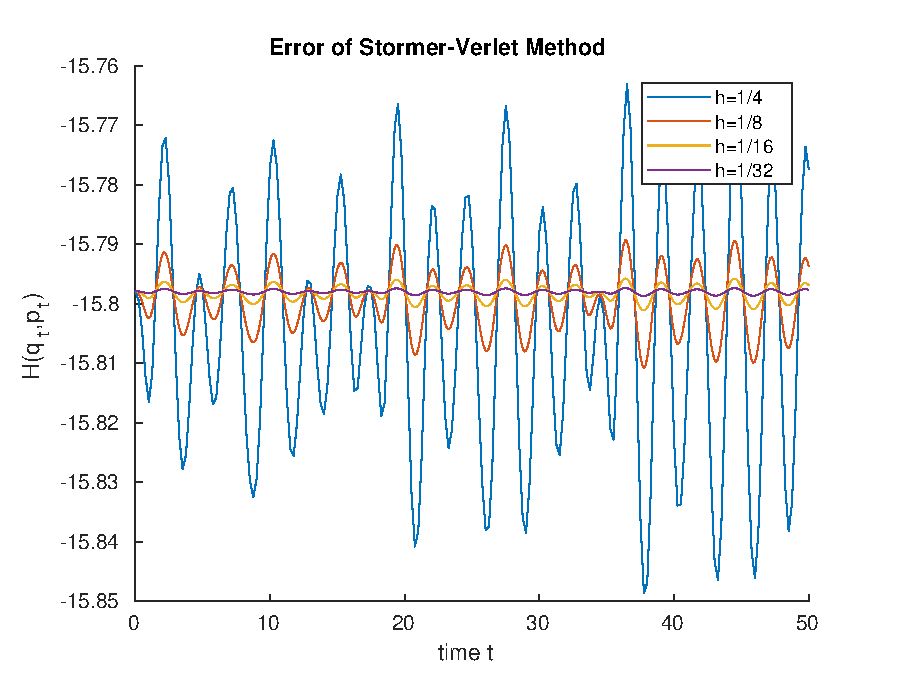
\includegraphics[width = 0.5\linewidth]{figures/phonationerr.eps}
	\caption{
		Evaluating the Hamiltonian for the model for phonation, integrated using the St\"ormer-Verlet method.
		Initial conditions are the same as that of Figure \ref{fig:phon}.
		The error of the method is shown to be $\mathcal{O}(h^2)$ in evaluating the Hamiltonian.
	}
	\label{fig:phonhamil}
\end{figure}

We move on to discuss results on the closeness of the Hamiltonian that corresponds to the problem solved by the numerical method.
This is an interesting result from backward error analysis.
If we can deduce that the modified Hamiltonian is sufficiently close to the original,
this merits the numerical solution in terms of preservation of quality.

Before considering the modified Hamiltonian, we need to introduce the concept of a generating function.
This methodology is covered in \cite{Casas_2016} in a wider analysis.
These are important when considering a change of coordinates.
First, recall Hamilton's equations
\begin{align*}
	&\dot{q}_i = \frac{\partial H}{\partial p_i}, &\dot{p}_i = \frac{- \partial H}{\partial q_i}.
\end{align*}
Define a new coordinate pair $Q_i = Q_i(q,p,t)$ and $P_i = P_i(q,p,t)$.
There must be another Hamiltonian $\tilde{H}$ which describes these transformed coordinates
\begin{align*}
	&\dot{Q}_i = \frac{\partial \tilde{H}}{\partial P_i}, &\dot{P}_i = \frac{- \partial \tilde{H}}{\partial Q_i}.
\end{align*}
This modified Hamiltonian tells us about the behaviour of the solution in this new coordinate system.
The motivation for this transformation is the aim of describing the behaviour of the system in a potentially simpler form using a different coordinate system. %is it?
There is a relation between these coordinates which is given by
\begin{equation}
	\sum_{i=1}^{d} p_i \mathrm{d}q_i - H \mathrm{d}t = \sum_{i=1}^{d} P_i \mathrm{d}Q_i - \tilde{H} \mathrm{d}t + \mathrm{d}F(q,p).
	\label{eqn:genfunc}
\end{equation}
This is an equation involving differential forms $\mathrm{d}q_i, \mathrm{d}t$, etc. but the key takeaway is the relationship involving the expression $\mathrm{d}F$ between coordinate systems.
The relationship between the Hamiltonians themselves is
\begin{equation*}
	\tilde{H}(Q,P,t) = H(q,p,t) + \frac{\partial F}{\partial t}.
\end{equation*}
We call $F$ a generating function. This is because the definition of $F$ can be used to reconstruct the coordinate transformation.
Note also that we wrote $\mathrm{d}F(q,p)$ on the original coordinates above, but if we know the transformation then we can write $F(q,p)$ and $F(Q,P)$ analogously by inverting the transformation.
This is because $F(Q,P) = F(Q(q,p),P(q,p))$.
We now introduce a result on the modified Hamiltonian.

\begin{theorem}[Hairer, Lubich, Wanner 2006]
Consider a generating function for a numerical method $\Phi_h(q,p)$ given by
\begin{equation}
	F(q,P,h) = h F_1(q,P) + h^2 F_2(q,P) + \mathellipsis
	\label{eqn:methodgen}
\end{equation}
where the functions $F_i$ are defined on some domain $D$ which is an open set.
The modified Hamilton's equations are 
\begin{align*}
	&\dot{q}_i = \frac{\partial \tilde{H}}{\partial p_i}, &\dot{p}_i = \frac{- \partial \tilde{H}}{\partial q_i}.
\end{align*}
where the modified Hamiltonian is
\begin{equation}
	\tilde{H}(q,p) = H(q,p) + h H_2(q,p) + h^2 H_3(q,p) + \mathellipsis
	\label{eqn:powerham}	
\end{equation}
where if the method is order $p$, then $H_i = 0$ for $i \leq p$.
The $H_i$ are defined and smooth on $D$.
Therefore, the closeness of the modified Hamiltonian to the original is $\mathcal{O}(h^p)$.
\end{theorem}

If this domain $D$ is the entire space of points $q,P$ then this result is globally defined, but over some restricted domain the result still holds but only locally.
A proof is given in \cite{gni2006}, but the result features in both and \cite{Casas_2016} gives examples.
The proof makes use of mixed-variable generating functions. If we have a generating function $F$ on $(q,P)$,
then
\begin{align*}
	&Q = \frac{\partial F}{\partial P}(q,P), &p = \frac{\partial F}{\partial q}(q,P).
\end{align*}
Furthermore, the proof requires a particular kind of generating function, being the function $\tilde{F}$ obtained from the solution of the Hamilton-Jacobi partial differential equation
\begin{equation*}
	\frac{\partial \tilde{F}}{\partial t}(q,P,t) = \tilde{H} \left(
		P, q + \frac{\partial \tilde{F}}{\partial P}(q,P,t)
	\right)
\end{equation*}
with initial condition $\tilde{S}(q,P,0) = 0$.
This detail is necessary, and more detail is given in \cite{gni2006}.
We now consider the proof for this result.
\begin{proof}
	Let $P,Q$ be the coordinates for the exact solution of the modified equation defined by the perturbed Hamiltonian $\tilde{H}$.
	We first want a generating function $\tilde{F}(q,P,t)$ defining the coordinate transformation.
	It is given (in the text) that if $\tilde{F}$ is a solution to the Hamilton-Jacobi PDE, then it is a unique solution which defines the map
	\begin{align*}
		&Q = q + \frac{\partial \tilde{F}}{\partial P}(q,P,t), &p = P + \frac{\partial \tilde{F}}{\partial q}(q,P,t).
	\end{align*}
	This is an expression involving $t$, and our numerical method is developed using the parameter $h$.
	We want $\tilde{F}$ here to match the expression $F(q,P,h)$ given in the statement of the theorem at $t=h$.
	We can start by considering $\tilde{F}$ as a series expansion around $t=h$, which will take the form
	\begin{equation*}
		\tilde{F}(q,P,t) = t \tilde{F}_1 (q,P,h) + t^2 \tilde{F}_2 (q,P,h) + \mathellipsis
	\end{equation*}
	If we plug this into the Hamilton-Jacobi PDE, we can compare powers of $t$ to obtain expressions for the terms in the series.
	The results come out by Taylor expansion in one dimension since $\tilde{H}$ evaluates at $P$.
	The first few terms are
	\begin{equation}
		\begin{aligned}
			\tilde{F}_1(q,P,h) &= \tilde{H}(q,P) \\
			2 \tilde{F}_2(q,P,h) &= \frac{\partial \tilde{H}}{\partial q}(q,P,h) \cdot \frac{\partial \tilde{F}_1}{\partial P}(q,P,h) \\
			\mathellipsis
		\end{aligned}
		\label{eqn:genh}
	\end{equation}
	The notation on the arguments is not important since these are just functions,
	but we stick with $(q,P)$ for consistency.
	We have expressions for $\tilde{F}_j$ in terms of derivatives of $\tilde{H}$,
	and we also have an expression for $\tilde{H}$ about $H$ in powers of $h$.
	If we let $\tilde{F}_j$ be \textit{another} series of the form
	\begin{equation*}
		\tilde{F}_j(q,P,h) = \tilde{F}_{j1}(q,P) + h \tilde{F}_{j2}(q,P) + h^2\tilde{F}_{j3}(q,P) + \mathellipsis
	\end{equation*}
	then we can use this expansion, and the expansion of $\tilde{H}$ in Equation \ref{eqn:powerham},
	both in powers of $h$,
	and match coefficients by plugging the terms into the entries in Equation \ref{eqn:genh}.
	Trivially, $\tilde{F}_{1k}(q,P) = H_k(q,P)$ from the first entry, so we have the original Hamiltonian plus a series in powers of $h$.
	For $j=2$, we get terms such as
	\begin{align*}
		2 \tilde{F}_{21}(q,P) &= \frac{\partial H}{\partial q}(q,P) \cdot \frac{\partial H}{\partial P}(q,P) \\
		2 \tilde{F}_{22}(q,P) &= \frac{\partial H_2}{\partial q}(q,P) \cdot \frac{\partial H}{\partial P}(q,P) + \frac{\partial H}{\partial q}(q,P) \cdot \frac{\partial H_2}{\partial q}(q,P) \\
		\mathellipsis
	\end{align*}
	In general for $j > 1$ we have that $\tilde{F}_{jk}(q,P)$ is a function depending on derivatives of $H_l$ for $l \leq k$\footnote{
		The book states $l < k$, however equality is attained, for example $\tilde{F}_{22}$ involves derivatives of $H_2$.
	}.
	Finally, recall the purpose of the generating function.
	The function $F(q,P)$ defines the numerical method.
	Therefore $\tilde{F}(q,P,h)$ needs to match $F(q,P,h)$ as defined in Equation \ref{eqn:methodgen}.
	We get the requirements
	\begin{align*}
		F_1(q,P) &= \tilde{F}_{11}(q,P) \\
		F_2(q,P) &= \tilde{F}_{12}(q,P) + \tilde{F}_{21}(q,P) \\
		\mathellipsis
	\end{align*}
	from comparing coefficients of $h$.
	Recall that we have $\tilde{F}_{1k}(q,P) = H_k(q,P)$ from the first row of Equation \ref{eqn:genh}.
	Therefore, the generating expression is a perturbation from the original Hamiltonian and we have
	\begin{equation*}
		F_j(q,P) = H_j(q,P) + \mathcal{D}_j(H_k(q,P))
	\end{equation*}
	where $\mathcal{D}_j$ is some function of derivatives of $H_k$ for $k \leq j$.
	This expression allows us to determine the $H_j$ given a generating function.
	
	Recall the definition of the generating function from Equation \ref{eqn:genfunc}. %logic is bad but it will have to do.
	Assume that the numerical method defined by the generating function $F$ is $\mathcal{O}(h^r)$.
	This generating function $F$ itself is the same order.
	Since we match terms in $F$ and $\tilde{F}$, both are $\mathcal{O}(h^r)$ i.e. the highest order term is $h^{r+1}$.
	Therefore, we must have that $\tilde{F}_{jk} = H_k = 0$ for $k \leq r$.

	Furthermore, since the $F_j$ are defined in terms of $H_j$, they must be defined on the same domain $D$.
\end{proof}

The direct implication is that a higher order method will converge faster to the true \textit{qualitative behaviour}.
Figure \ref{fig:phonhamil} shows the phonation problem from earlier.
We evaluate the Hamiltonian using its closed form expression using the numerical solution generated by the St\"ormer-Verlet scheme.
As we can see, the perturbed Hamiltonian approaches the unmodified Hamiltonian by $\mathcal{O}(h^2)$, the order of the method.

\section{Applications}

\subsection{Example - The Three-Body Problem}

\begin{figure}
	\centering
	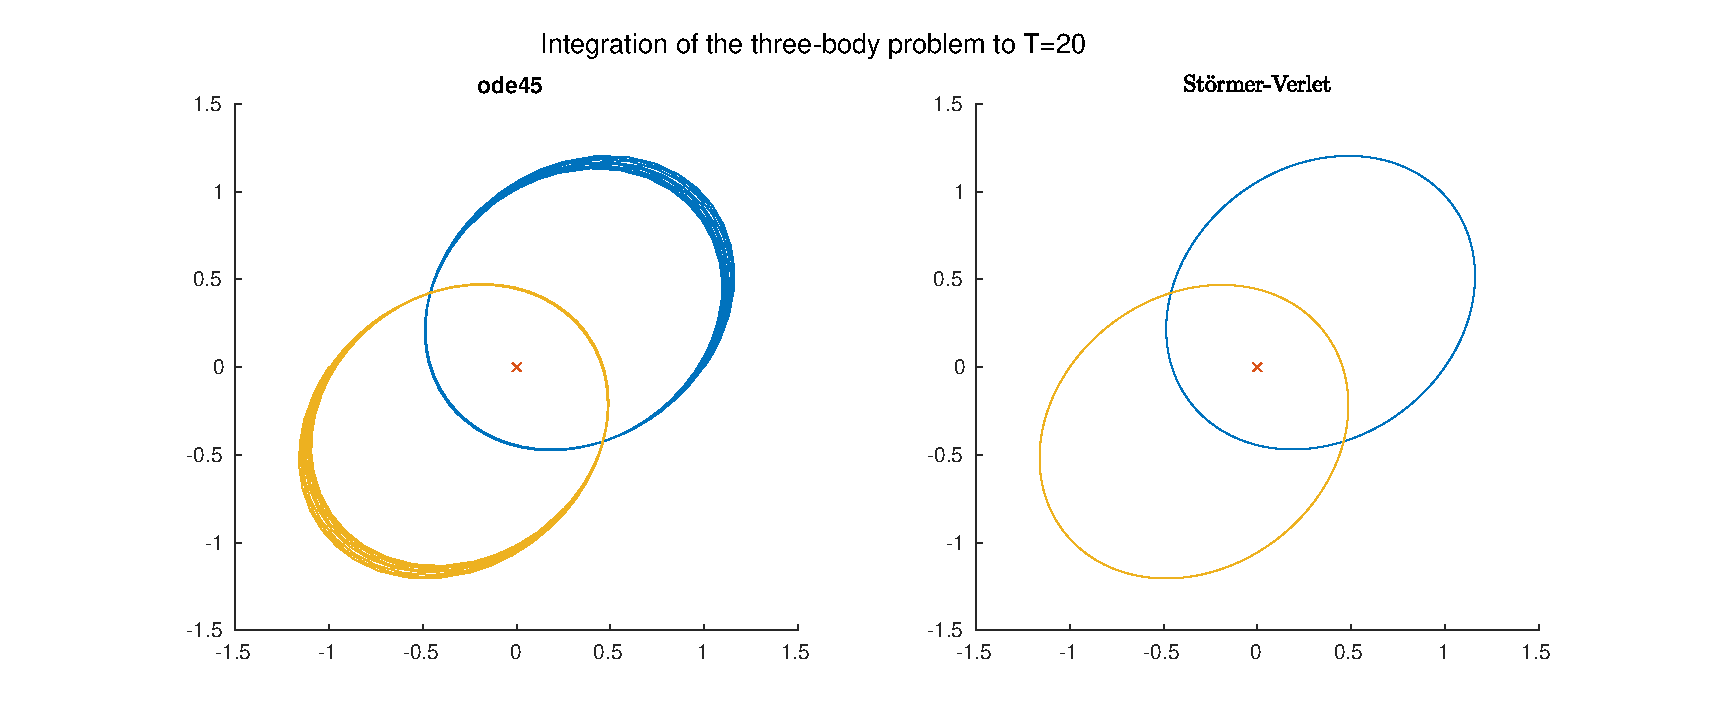
\includegraphics[width=\linewidth]{Matlab/threebodyorbit}
	\caption{
		Integration of the three-body problem for a timespan $t \in [0, 20]$.
		Initial conditions are configured to construct an orbit.
		Two masses orbit a stationary third mass at the origin.
		Initial conditions on the $y=0$ line at $(1,0)$, $(0,0)$ and $(-1,0)$.
		Initial momentum is rotationally symmetric, approximately $(0.35, 0.53)$ at $(1,0)$.
	}
	\label{fig:threebody}
\end{figure}

The three-body problem \cite{musielak2014three} is a huge point of interest in celestial mechanics.
It describes the motion of three point-masses in a closed system which move under gravitational acceleration to each other.
An important subclass is the \textit{restricted} three-body problem, in which one mass is relatively large in magnitude, and can be regarded as fixed compared to the other two bodies.
The restricted three-body problem can be used to model the motion of the earth and moon relative to the sun.

The classical form of the dynamics for the three-body problem is
\begin{equation*}
	\begin{aligned}
		\ddot{x}_1 &= -G m_2 \frac{x_1 - x_2}{|x_1 - x_2|^3} - -G m_3 \frac{x_1 - x_3}{|x_1 - x_3|^3} \\
		\ddot{x}_2 &= -G m_3 \frac{x_2 - x_3}{|x_2 - x_3|^3} - -G m_1 \frac{x_2 - x_1}{|x_2 - x_1|^3} \\
		\ddot{x}_3 &= -G m_1 \frac{x_3 - x_1}{|x_3 - x_1|^3} - -G m_2 \frac{x_3 - x_2}{|x_3 - x_2|^3}
	\end{aligned}
\end{equation*} 
where $x_i$ is the vector position of the point-mass particle with mass $m_i$.
In Hamiltonian form \cite{musielak2014three}, this is the problem
\begin{align*}
	&\dot{q}_i = \frac{\partial H}{\partial p_i}, &\dot{p}_i = \frac{- \partial H}{\partial q_i}.
\end{align*}
where
\begin{equation*}
	H(q,p) = - \frac{G m_1 m_2}{|q_1 - q_2|} - \frac{G m_2 m_3}{|q_2 - q_3|} - \frac{G m_3 m_1}{|q_3 - q_1|} + \frac{p_1^2}{2m_1} + \frac{p_2^2}{2m_2} + \frac{p_3^2}{2m_3}.
\end{equation*}
for particles with position $q_i$ and momentum $p_i$.

See Figure \ref{fig:threebody} for a visualisation of the trajectories of the three body problem under a particular set of initial conditions.
The integration from \texttt{ode45()} shows clear drift from the original path of the orbit.
A very high relative tolerance of $10^{-12}$ was used for this method, so this is arguably the best approximation we can hope to compute with an explicit method.
In comparison, the St\"ormer-Verlet scheme is only second order accurate, but we are able to maintain the path of orbit over the same timespan because it is a symplectic method.
Any deviation from the orbit path is not visible.

See Appendix \ref{apn:ham} for implementations and tests of symplectic integration schemes.

\subsection{Review}

We have given an overview of the structure of problems in Hamiltonian mechanics and how the property of symplecticity is directly related.
We have introduced several symplectic integration methods and the theory behind them.
We have demonstrated these with examples to show the utility of these methods.
It is clear that when the nature of the Hamiltonian is important to the behaviour of the problem, it would be beneficial to use a symplectic method.

Symplectic integration is extremely prevalent in celestial mechanics, where we may need to integrate a Hamiltonian system over a long timespan in order to estimate the motion of celestial bodies far into the future.
The three-body problem is a simple but insightful demonstration of problems such as these.
Other applications in physics are molecular dynamics and particle physics.

Having covered symplectic integration, the theory for which is extremely prevalent and researched,
we now move on to the field of positivity preservation, which is a much more recent and unclear area of geometric numerical integration.

% error control on explicit method versus symplectic method - what is the cost

